\usepackage{}% LLNCS macro package for Springer Computer Science proceedings;
% Version 2.20 of 2017/10/04
%
\documentclass[runningheads]{llncs}
%
\usepackage{graphicx}
\usepackage{lipsum}
\usepackage{amsmath}
\usepackage{authblk}
\usepackage{makecell,array}
%\usepackage{natbib}
%\usepackage[square,sort,comma,numbers]{natbib}
%\usepackage[numbers]{natbib}

\usepackage[square,numbers]{natbib}
\usepackage{graphicx}
\usepackage{float}
\usepackage{gensymb}
%\setcounter{secnumdepth}{3}
% Used for displaying a sample figure. If possible, figure files should
% be included in EPS format.
%
% If you use the hyperref package, please uncomment the following line
% to display URLs in blue roman font according to Springer's eBook style:
% \renewcommand\UrlFont{\color{blue}\rmfamily}

\begin{document}
	%
	\title{Bidirectional Transformations between specifications languages for Runtime Verification}
	%
	%\titlerunning{Abbreviated paper title}
	% If the paper title is too long for the running head, you can set
	% an abbreviated paper title here
	%
	\author{Lisandra Silva a73559@uminho.pt}
	%
	% First names are abbreviated in the running head.
	% If there are more than two authors, 'et al.' is used.
	%
	\institute{National Institute of Informatics, Tokyo Japan\\}
	%
	\maketitle              % typeset the header of the contribution
	
	\begin{abstract}
		Use of Bidirectional Transformations to synchronize different specifications for Runtime Verification. More specifically to synchronize a specification expressed as a Regular Expression and another expressed as a Finite State Machine.
	
		\keywords{Bidirectional Transformations  \and Runtime Verification \and Regular Expressions \and Non-deterministic Finite Automata \and Deterministic Finite Automata}
	\end{abstract}
	%
	%
	%
	\section{Introduction}

\subsection{Motivation}
There a few different specifications languages to specify monitors, and comparing the expressiveness is these languages is not straightforward. Besides, sometimes it is not easy to select a specific language to write a specification, because the syntax and operations of a particular language may make certain specifications easier or harder to write and/or read. 

	\par
	
    	\section{Runtime Verification}
	\textit{Runtime Verification} (RV) is a dynamic analysis method aiming at checking whether a run of the system under scrutiny satisfies a given correctness property.

  \begin{figure}
	\centering
	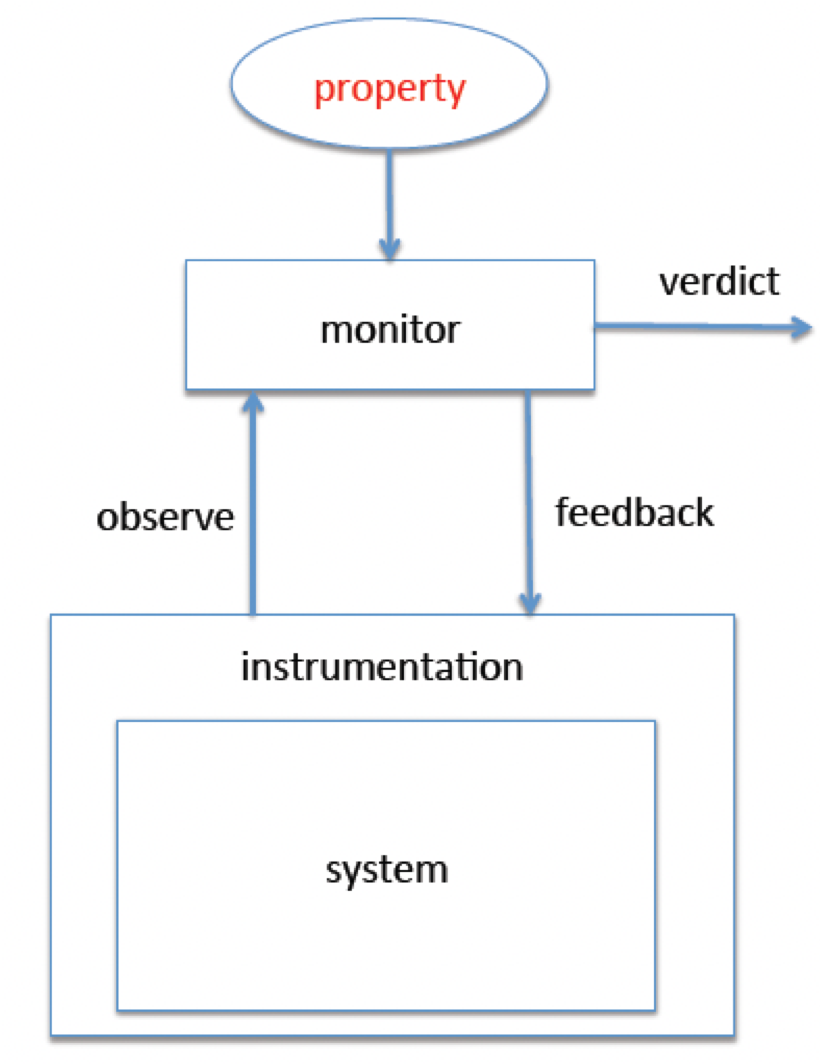
\includegraphics [scale=0.4]{Images/rv.png}
	\caption{An overview of the RV process}
	\label{rv}
\end{figure}

 The components of a RV environment are the system to be checked and a set of properties to be checked against the system execution. Properties can be expressed in a formal specification language, or even as a program in a general-purpose programming language. From a given property, a monitor is generated, i.e., a decision procedure for that property - \textit{monitor synthesis}. The system is instrumented to generate the relevant events to be fed into the monitor - \textit{system instrumentation}. In the next step, the system's execution is analyzed by the monitor - \textit{execution analysis}. The monitor is able to consume the events produced by the running system and, for each consumed event, emits a verdict indicating the status of the property, depending on the event sequence seen so far. Finally, the monitor sends feedback to the system so that more specific corrective actions can be taken (Figure \ref{rv}) ~\cite{rvart}.
 
 
\subsection{Formal Specification of the system behaviour}
There are different formal approaches to describe the expected behaviour of a system. But before presenting some different specification languages, let first present some general properties of these formalisms. 

\subsubsection{Events}
The behaviour of a system can be analyzed as the way the system changes over time, and this can be done through its observation. To abstract these observations we will use \textit{Events} - discrete atomic entities that represent \textit{actions} or \textit{state changes} made by the system. 
The system's observable events of interest is called its \textit{alphabet}. The choice of events is part of the specification and will determine the available information about the system and about what properties can be described.

\subsubsection{Traces}
A \textit{trace} is a sequence of events and abstract the behaviour of a single run of the system. Obviously an observable trace must be finite, but it is sometimes useful to think about the possible infinite behaviours of a system, therefore, a trace can be viewed as a finite prefix of the infinite behaviour.

\subsubsection{Properties and Specifications}
The abstraction of a property can be described as a set of traces and its specification is a concrete (textual) object that denotes this set of traces.
As there are many specifications languages, one can have many specifications for a single property, but a property is unique and independent of the specification language. If the specification language is ambiguous, then the specific property may not be clear. Dealing with such ambiguities is a common issue in the specification process ~\cite{rv2}.


\subsection{Different language specifications}
This section presents a brief description of the main specification languages for RV, as well as some of their general features.

A RV specification language can be \textit{Executable} if the specification is directly executable and therefore more low-level, or \textit{Declarative} in which an executable object (monitor) is generated from the specification. Also, some specification languages are more suited to specify sets of finite traces whereas others are more suited to specify infinite traces. A specification may also capture \textit{good} or \textit{bad} behaviour. A match against a good behaviour specification represents \textit{validation} of the desired property, whereas a match a bad behaviour specification represents \textit{violation} of that property ~\cite{rv2}.

\subsubsection{Regular Expressions}
Familiar declarative language in Computer Science for describing sets of strings, but can also be used in RV to describe traces of events, where the atoms are not characters but events. The regular expression matches if any \textit{suffix} of the trace matches the expression - \textit{suffix-matching} - to attest the validation or violation of the property (e.g., in the work of TraceMatches) ~\cite{rvart}.

\subsubsection{Finite State Machines}
These type of specifications have the advantage of being directly executable, in opposition to regular expressions and temporal logic, since both require \textit{monitor synthesis} to produce a monitor, which is usually described as some form of state machine. 

\vspace{5mm}

The formalisms of \textbf{Linear Temporal Logic} and \textbf{Context Free Grammars} can also be used for specifications in RV, but since they are not the main focus of the present work they will not be further approached. 



	
    \section{Regular Expressions and Finite State Machine}

\subsubsection{Thompson's algorithm}
	
	\subsubsection{Glushkov's algorithm}
	
	\subsubsection{Powerset construction algorithm}
	
	\subsubsection{Kleen's Algorithm}
	
	\section{Bidirectional Transformations}
	
	\section{Implementation}
	\subsection{Reasoning about BX}
	
	\subsection{Get function from RE to NDFA}
	
	\subsection{Get function from NDFA to DFA}
	
	\subsection{Put back function from DFA to NDFA}
	
	\section{Future work}
	
	
	
	
	
	
	\iffalse
	\section{Regression based approach for link residual time prediction(RLRP)}
	MANET is infrastructure less network form by mobile nodes. These mobile nodes communicate to each other via single hop or multiple hops. Mobility is a key attribute, this causes route failure because the topology of the network changes frequently. So for predicting the future of network topology, link residual time prediction is an important field.
	\par 
	Proposed approach is based on column Mobility Model ~\cite{r15} of mobile nodes it assumes that each node broadcast hello packets to inform its availability in the range. When neighbour node receives hello packet from a sender it uses its signal strength (RSSI Value) to estimate the distance between them.
	------
	monotonically decreasing sequence of RSSI indicates that nodes are moving away from each other and link between them may break down in future. -----.
	\par
	Regression-based approach for link residual time prediction(RLRP) is based on least square polynomial regression. Regression is a better approach than interpolation ~\cite{r16} because interpolation looks for the predicted form of function but in regression looks for a function that minimizes error, this needs a good approximation. 
	
	The following steps are discussed below: 
	
	\begin{enumerate}
		\item Let node $i$ and $j$ are any two neighbour nodes of MANET.
		\item Node $i$  broadcasts hello packets of constant predefined signal strength at periodic intervals.
		\item Neighboring node $j$ receives these packets and  maintains a record of RSSI (received signal strength indication) and packet arrival time in a table. RSSI is a measurement of the signal strength in recieved radio signal. Let $RSSI_{i,j_{1}},RSSI_{i,j_{2}},......RSSI_{i,j_{m}}...\\
		.....RSSI_{i,j_{n}}$ are signal strengths of recieved hello packets by  $j$th node transmitted from  $i$th node recieved at time  $t_{i,j_{1}},t_{i,j_{2}},......t_{i,j_{m}}.....t_{i,j_{n}}$ respectively.
		\item When node $j$ observes a monotonically decreasing pattern of received signal strengths of hello packets as in equation~\ref{eqn:rssi}; In considered case let $m$th onward packets have monotonically  decreasing RSSI valuues then:
		\begin{equation}
		\label{eqn:rssi}
		RSSI_{i,j_{m}}>RSSI_{i,j_{m+1}}>RSSI_{i,j_{m+2}}.....>RSSI_{i,j_{m+n}}
		\end{equation}
		A set ${\Re}_{i,j}$ as equation~\ref{eqn:set} is formulated with above monotonically decreasing hello packet signal strengths and times as elements.
		\begin{equation}
		\label{eqn:set}
		{\Re}_{i,j}= \left\lbrace (RSSI_{i,j_{m}},t_{i,j_{m}}),(RSSI_{i,j_{m+1}},t_{i,j_{m+1}}), \\
		...,(RSSI_{i,j_{m+p}},t_{i,j_{m+p}})...\\
		,(RSSI_{i,j_{m+n}})\right\rbrace 
		\end{equation}
		
		\item Least square polynomial regression based link failure prediction module is invoked.
		\begin{itemize} 
			\item Following is the representation of quadratic model which relates elements of set ~\ref{eqn:set}.
			\begin{equation}% ##-- EQUATION TEMPLATE --##
			\begin{aligned}
			\left[\begin{matrix}RSSI_{i,j_{m}} \\RSSI_{i,j_{m+1}}\\ \vdots\\RSSI_{i,j_{m+p}}\\ \vdots\\RSSI_{i,j_{m+n}}
			\end{matrix} \right] = \left[\begin{matrix} t^{2}_{m} & t_{m} & 1\\t^{2}_{m+1} & t_{m+1} & 1\\   \vdots & \vdots & \vdots\\t^{2}_{m+p} & t_{m+p} & 1 \\  \vdots & \vdots & \vdots  \\t^{2}_{m+n} & t_{m+n} & 1 \end{matrix} \right] 
			*\left[\begin{matrix}  a_{ij} \\ b_{ij} \\ c_{ij}\end{matrix} \right]             
			\end{aligned}\label{eq:six}
			\end{equation}
			\item Equation:~\ref{eq:seven} is simplified representation of equation:~\ref{eq:six}. 
			\begin{equation}% ##-- EQUATION TEMPLATE --##
			\begin{aligned}
			\varUpsilon_{ij}     = \varPhi_{ij} *\varTheta _{ij}
			\end{aligned}\label{eq:seven}
			\end{equation}     
			where 
			\begin{equation}% ##-- EQUATION TEMPLATE --##
			\begin{aligned}
			\varUpsilon_{ij} =\left[\begin{matrix}RSSI_{i,j_{m}} \\RSSI_{i,j_{m+1}}\\ \vdots\\RSSI_{i,j_{m+p}}\\ \vdots\\RSSI_{i,j_{m+n}}
			\end{matrix} \right] , \varPhi_{ij} =\left[\begin{matrix} t^{2}_{m} & t_{m} & 1\\t^{2}_{m+1} & t_{m+1} & 1\\   \vdots & \vdots & \vdots\\t^{2}_{m+p} & t_{m+p} & 1 \\  \vdots & \vdots & \vdots  \\t^{2}_{m+n} & t_{m+n} & 1 \end{matrix} \right] ,       \varTheta _{ij}=\left[\begin{matrix}  a_{ij} \\ b_{ij} \\ c_{ij}\end{matrix} \right] 
			\end{aligned}\label{eq:eight}
			\end{equation} 
			\item Least Square estimate ~\cite{r17} $\hat{\varTheta_{ij}}$ of vector parameter $\varTheta _{ij}$ of equation:~\ref{eq:seven} is following: 
			\begin{equation}% ##-- EQUATION TEMPLATE --##
			\begin{aligned}
			\hat{\varTheta_{ij}}={(\varPhi^{T}\varPhi)}^{-1}\varPhi^{T}\varUpsilon_{ij}
			\end{aligned}\label{eq:eight}
			\end{equation} 
			\item In this way one can estimate values of $\hat{a}_{ij}$,$\hat{b}_{ij}$ and $\hat{c}_{ij}$ and express  signal strength  of $i\Leftrightarrow j$th link $RSSI_{ij}$. Equation:~\ref{eq:nine} represents best fit quadretic polynomial of signal strength with respect to time.
			\begin{equation}% ##-- EQUATION TEMPLATE --##
			\begin{aligned}
			RSSI_{ij} = \hat{a}_{ij} t^{2} + \hat{b}_{ij}t + \hat{c}_{ij}
			\end{aligned}\label{eq:nine}
			\end{equation}        
			\item By antenna characteristics threshold value of signal strength $RSSI_{thresh}$ ~\cite{r12} , min signal strength rquired  to be detected by reciever antenna is a known parameter. Solution of equation:~\ref{eq:ten} will provide estimate of time$\tau_{i,j_{break}}$ when link will break. 
			\begin{equation}% ##-- EQUATION TEMPLATE --##
			\begin{aligned}
			RSSI_{thresh} = \hat{a}_{ij} t^{2} + \hat{b}_{ij}t + \hat{c}_{ij}
			\end{aligned}\label{eq:ten}
			\end{equation}    
			Value of $\tau_{i,j_{break}}$ can be calculated with help of Sridharacharya formulae ~\cite{r13}.
			\begin{equation}% ##-- EQUATION TEMPLATE --##
			\begin{aligned}
			\tau_{i,j_{break}} =\frac{-\hat{b}_{ij} \pm \sqrt{\hat{b}_{ij}^{2}-4\hat{a}_{ij}\hat{c}_{ij}}}{2\hat{a}_{ij}}
			\end{aligned}\label{eq:eleven}
			\end{equation}            
			
			This computed value $\tau_{i,j_{break}}$ is the estimated time when link between $i_{th}$ and $j_{th}$ node will break.  
		\end{itemize}
		\item When Current time= $\tau_{i,j_{break}}- \delta$,  where $\delta$ is very small time; corrective action is taken to prevent packet drop.    
		
		
	\end{enumerate}
	
	
	
	
	
	\section{ Simulation Results and Analysis}
	The proposed approach is based on AODV routing protocol. NS-2.35 ~\cite{r14} tool is used for simulation. NS2.35 is an open source tool which is used for research in networking. 
	
	\subsection{Experimantal setup}
	Column Mobility Model ~\cite{r15} is used for representing mobility of node. In column mobility model, a set of mobile nodes are moving linearly from one location to another location. Velocity of nodes varies from 2 m/s to 10m/s. The simulation area is 500*500, omni-direction antenna model and two-way ray ground radio propagation model are used. In Table~\ref{tab1} detailed parameters for simulation are summarized.
	
	
	\begin{table}
		\caption{Simulation parameters}\label{tab1}
		
		
		\begin{center}
			\begin{tabular}{|c c |} 
				\hline
				Parameters & Values \\ [0.5ex] 
				\hline\hline
				Size & 500 m by 500 m  \\ 
				\hline
				Simulation Time & 500 s \\
				\hline
				Velocity & 2,4,6,8,10 m/s \\
				\hline
				Packet length & 512 bytes \\
				\hline
				Traffic pattern & TCP\\ [1ex] 
				\hline
				MAC protocol & IEEE 802.11  \\ [1ex] 
				\hline
				
				
			\end{tabular}
		\end{center}
		
		
	\end{table}
	
	\subsection{Analysis of results}
	\begin{table}
		\caption{Comparision of estimated vs actual link residual time }\label{tab2}                        
		\begin{center}
			\begin{tabular}{|c c c|} 
				\hline
				Link No & Estimated Residual Time & Actual Residual time  \\   
				\hline\hline
				1 & 252.2639 sec  & 251.9715 sec \\ 
				%                    \hline
				2 & 227.7949 sec  & 226.4358 sec \\
				%                    \hline
				3 & 209.076 sec & 207.9343  sec \\
				%                    \hline
				4 & 204.8224 sec & 204.0284 sec \\
				%                    \hline
				5 & 168.5515 sec & 167.4681 sec \\
				%                    \hline
				6 & 97.8936 sec & 96.5896 sec  \\  
				\hline                    
			\end{tabular}
			
		\end{center}    
	\end{table}    
	Table~\ref{tab2} is representing a comparison of estimated link residual time with actual link residual time for a 5 node manet with node velocity 2m/sec. On observing the data one can conclude that the present algorithm is generating remarkable performance in terms of accurate estimation of link residual time.
	
	\par Root-mean-square error (RMSE) of link residual time  calculated  as following equation:~\ref{eq:e1}is chosen as performance measure:
	\begin{equation}% ##-- EQUATION TEMPLATE --##
	\begin{aligned}
	RMSE_{v}=\sqrt{\dfrac{1}{L}\sum_{k=1}^{L} (\tau_{k,v_{break}}-\tau_{k,v_{actual}})^{2}}
	\end{aligned}\label{eq:e1}
	\end{equation} 
	where    $RMSE_{v}$ is  Root-mean-square error (RMSE) of link residual time at node velocity $v$m/sec, $\tau_{k,v_{break}}$ and  $\tau_{k,v_{actual}}$ are estimated and actual link residual times of any $k_{th}$ link of MANET of total $L$ links with node velocity $v$ respectivey.        
	
	
	\par
	Fig:~\ref{Fig1} shows the comparison of RMSE for the different sets of n points with monotonically decreasing pattern of received signal strengths of hello packet used in the least square polynomial regression wrt velocity of nodes. It can be concluded that increasing node velocity is not directly affecting RMSE value of link residual time; means estimated link residual time is immune to node velocity scaling. 
	\par
	There are three different curves showing RMSE vs node velocity relationship with varying number of hello packets of monotonically decreasing RSSI appearing in the figure:~\ref{Fig1}. It can be concluded that with an increasing value of $n$ there is again in RMSE value of error but since computational overhead is also increasing with $n$. Hence in this algorithm, an optimal value $n=5$ has been chosen.
	
	
	\begin{center}
		\begin{figure}
			
			\includegraphics[width=11cm, height=5.5cm]{r1.jpg}
			\caption{RMSE vs node velocity} \label{Fig1}
			
		\end{figure}
	\end{center}
	\par    
	Fig.~\ref{Fig2} shows a comparison between regression and interpolation based approaches of link residual time estimation. From the figure, it can be concluded that by adapting regression-based approaches one can have an edge over interpolation based approaches. Mathematically, regression-based approaches uses a polynomial pattern within considered points; means there is no guarantee that polynomial will pass through at least one chosen point. On the other hand, interpolation provides curve fitting type solution; means it is guaranteed that a $n_{th}$ degree polynomial will pass through n selected points. In this, although it is guaranteed that there will be zero error at considered n points but for other points in the domain this polynomial will not provide a solution with the optimal error.
	Although in both cases this polynomial is extrapolated as in equation:~\ref{eq:ten} to find a solution for link residual time, yet the regression polynomial is better approximated for this point.
	
	
	\begin{center}
		\begin{figure}
			
			\includegraphics[width=11cm, height=5.5cm]{r2.jpg}
			\caption{Comparision between RMSE of Interpolation vs Regression based residual time estimation} \label{Fig2}
			
		\end{figure}
	\end{center}
	
	%\begin{table}
	%    \caption{Predicted link residual time and actual link failure time when node velocity is 2 m/sec}\label{tab2}
	%    \begin{tabular}{|l|l|l|}
	%        \hline
	%        Heading level &  Example & Font size and style\\
	%        \hline
	%        Title (centered) &  {\Large\bfseries Lecture Notes} & 14 point, bold\\
	%        1st-level heading &  {\large\bfseries 1 Introduction} & 12 point, bold\\
	%        2nd-level heading & {\bfseries 2.1 Printing Area} & 10 point, bold\\
	%        3rd-level heading & {\bfseries Run-in Heading in Bold.} Text follows & 10 point, bold\\
	%        4th-level heading & {\itshape Lowest Level Heading.} Text follows & 10 point, italic\\
	%        \hline
	%    \end{tabular}
	%    \end{table}
	
	
	
	
	
	\section{Conclusion}
	The authors have presented a novel approach for link residual time prediction based upon cross-layer optimization and least square quadratic regression. Although these approaches are very powerful tools of contemporary researchers of networking community yet there are very limited examples of simultaneous use of both for link residual time prediction. Results are very promising and the algorithm is very simple in terms of implementation.
	
	\fi
	
	
	% ---- Bibliography ----
	%
	% BibTeX users should specify bibliography style 'splncs04'.
	% References will then be sorted and formatted in the correct style.
	%
	\bibliographystyle{apalike}
	\bibliography{mybib}
	%
	
\end{document}
